\chapter{直感的にツリーを作成できるインターフェース}
本章では直感的にツリーデータを入力する手法について述べる.

\section{主な機能}
試作するシステムでは,プロジェクトを「ミッション」と呼ぶ.
ユーザーは任意にミッションを作成することができ,ミッションごとに直感的なGUIでタスクツリーを構築することができる.
タスクには進捗状況の指定,タグの指定,コメント機能,編集履歴,ファイル添付をすることができる.
作成したミッションは任意のタイミングで一般公開することができるので,公開されたミッション間から後述するアルゴリズム類似ミッションを推定し,ユーザーに推薦することにより,組織を越えた協働を促進する.

\subsection{動作画面}
システムの動作画面を\ref{img:intereface_capture}に示す.

\begin{figure}[t]
	\begin{center}
		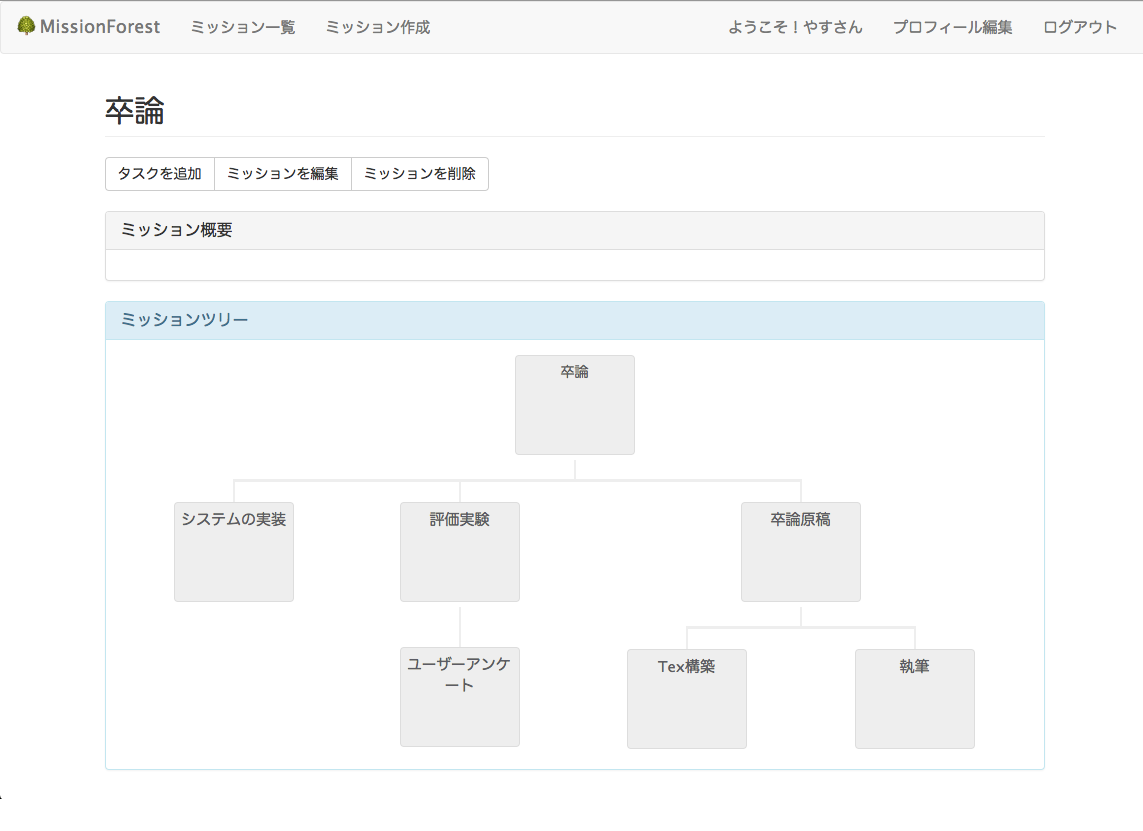
\includegraphics[width=0.9\linewidth]{assets/img/interface_capture.png}
		\caption{動作画面}
		\label{img:intereface_capture}
	\end{center}
\end{figure}

\section{ツリーエディタ}
直感的なツリーエディタGUIを作成するため,本研究で使用したJavaScriptライブラリを述べる.

\subsection{OrgChart}
\footnote{https://github.com/dabeng/OrgChart}
TODO: レイアウトアルゴリズムの説明
